\chapter{Entstehung und Grundgedanken}


Flow Design ist aus der Clean Code Development  (CCD) Bewegung heraus entstanden. Hauptinitiator und Erfinder ist Ralf Westphal.
Ralf Westphal war auch Mitbegründer und Miterfinder der Clean Code Development Bewegung.

\abk{CCD}{Clean Code Development } 

Clean Code Development ist eine Ansammlung aus Prinzipien, die einem helfen
sollen sauber programmierte Software zu schreiben. Diese Prinzipien sind aus dem Buch \enquote{Clean Code} von Robert C. Martin entnommen. Sauber programmierte Software hat 
die vor allem die Eigenschaft, dass Änderungen und Erweiterungen an ihrer Funktionalität
leicht zu realisieren sind. Laut Robert C. Martin\footnote{TODO:Buch und Seite angeben} gibt es in der Softwareentwicklung
keine Garantie dafür, dass sich eine für die Software relevanten
Rahmenbedingungen nicht jederzeit plötzlich ändern können. Sauber programmierte
Software kann leichter auf solche Änderungen angepasst werden. 

Es bedarf zwar anfänglich mehr Zeit ein Feature zu implementieren, dass den CCD Prinzipien entspricht, auf langer
Sicht jedoch steigt dieser Zeitaufwand nicht mit jedem neuen Feature stark
an. Im Vergleich dazu steigt bei einer unsauber programmierten Software der Zeitaufwand ein neues
Feature zu implementierten mit der Anzahl an bereits implementieren Features
exponentiell an \footnote{Clean Code Buch, Seite xx}. Irgendwann erreicht der Quellcode der Software dann einen Punkt, an
dem der Zeitaufwand ein neues Feature zu implementieren derart groß geworden ist, dass es besser ist die Software neu zu schreiben, anstatt sie anzupassen.

CCD bezeichnet eine saubere programmierte Software aus diesem Grund auch als \emph{evolvierbar}\footnote{\url{http://clean-code-developer.de/das-wertesystem/\#Evolvierbarkeit}}.
Software die mit dem Fokus auf Evolvierbarkeit hin programmiert wurde,
kann leicht an neue Rahmenbedingungen oder Kundenwünsche angepasst werden.


Eine weitere Eigenschaft von sauber programmierter Software ist dass sie gut zu
lesen ist und möglichst ohne Kommentare verstanden werden kann.
Programmcode wird öfters gelesen als geschrieben. Aus diesem Grund sind gute
Lesbarkeit eine wichtige Eigenschaft. Gute Lesbarkeit ist auch dann von großer
Bedeutsamkeit, wenn eine andere Person den Programmcode nachvollziehen muss, als diejenige Person, die ihn geschrieben hat.
Somit ist in größeren Softwareprojekten ein saubere Codebasis umso unverzichtbarer.

Prinzipien haben jedoch die Eigenheit, dass sie nicht so leicht einzuhalten sind wie konkrete Regeln.
Somit ist es in der Praxis schwer die Prinzipien auf den eigenen Code anzuwenden.
Hierbei soll Flow Design einen Lösungsansatz bieten. Flow Design bieten in
Ergänzung zu den CCD Prinzipien eine Entwurfsmethodik und dazugehörende Implementierungsregeln, die
die einfach zu befolgen sind und man erhält fast automatisch einen Code, der ein Großteil der CCD Prinzipien erfüllt.

\section{CCD Prinzipien}

Flow Design legt den Schwerpunkt vor allem auf folgende Prinzipien von CCD \footnote{\url{http://clean-code-developer.de/die-grade/roter-grad/}}:

\bigskip



\begin{table}[H]
	\centering
	\begin{tabular}{ | p{5cm} | p{9.5cm} | } 
	\hline
	KISS \linebreak (Keep It Stupid Simple)  & Ein System sollte so einfach wie möglich gestaltet werden. \\
	\hline
	YAGNI  \linebreak (You Ain't Gonna Need It) & Es soll nicht unnötig viel Zeit damit verbracht werden für zukünftige Eventualitäten zu programmieren. 
	Der Fokus sollte darauf liegen, was aktuell wirklich benötigt wird. \\
	\hline
	Lose Koppelung & Separate Einheiten eines Systems sollen über nur möglichst  wenige Punkte miteinander kommunizieren. \\
	\hline
	Orthogonalität & Änderungen an einer Funktion des Systems sollen auf so wenig wie möglich andere Funktionen des Systems negativen Einfluss haben. \\
	\hline
	\end{tabular}
	\medskip
	\caption{CCD Prinzipien}
\end{table}

\subsubsection{KISS}
\abk{KISS}{Keep It Stupid Simple} 

Die Komplexität der Lösung eines Problems soll immer in Relation zu der
Komplexität des Problems stehen.

Schnell passiert es, dass man die einfachste Lösung für ein Problem übersieht und das Problem unnötig verkompliziert.
Das KISS Prinzip soll einen in erster Linie ein Bewusstsein dafür schaffen bei
komplizierten Lösungen innezuhalten und sich nochmal genau zu
überlegen, ob es nicht eine einfachere Lösung gibt.
Manche Problemdomänen erfordern jedoch eine komplexe Lösung, da das Problem
komplex ist.

Verkomplizierte Lösungen müssen am besten schon beim Entwurf erkannt werden.
Hierbei soll Flow Design als Entwurfsmethode helfen, die einfachste und leicht
verständlichste Lösung für ein Problem zu finden.

\subsubsection{YAGNI}
\abk{YAGNI}{You Ain't Gonna Need It}  

Vielen Softwareentwickler ist es wohl schon passiert, dass sie es zu gut gemeint
haben mit dem vorausschauendem Denken. Etliche Funktionen wurden für ein
zukünftiges Szenario implementiert oder verkompliziert, die jedoch nie
eintrafen, oder falls sie eintrafen kam es anders als gedacht, oder die Software
wurde bereits durch eine andere ersetzt.
YAGNI soll einem das Bewusstsein dafür schärfen, wann man sich gerade mit einer
Situation beschäftigt, die die aktuellen Rahmenbedingungen überschreiten.
Man sollte sich eher auf das aktuelle Szenario beschränken und keine unnötige Ressourcen für zukünftige
Eventualitäten verschwenden.
Flow Design bietet hierfür Implementierungsregeln, die es einem ermöglichen
schnell Änderungen am Code zu realisieren.
Diese Eigenschaft des Codes bietet damit die Basis diesem Prinzip auch getrost
zu befolgen und sich auf die aktuellen Rahmenbedingungen zu konzentrieren.

\subsubsection{Lose Koppelung}

Ein System soll aus möglichst voneinander unabhängigen Untersystemen bestehen,
die nur über eine  klar definierte Stelle miteinander kommunizieren.
Bei jedem Aufruf einer Funktion oder Abrufen einer Variable entsteht eine
Koppelung zwischen beiden.
Ändert sich die Struktur des Codes, so muss jede Stelle angepasst werden, die zu
der geänderten Struktur eine Koppelung besitzt. Mit loser Koppelung möchte man
veranschaulichen, dass wenn eine Koppelung nötig ist, diese an einer Stelle konzentriert sein soll und
sich nicht an verschiedenen Stellen des Codes fortpflanzen soll.
Flow Design fördert das Entkoppeln und zeigt Abhängigkeiten bereits bei der Modellierung.

\subsubsection{Orthogonalität}

In einem dreidimensionalen Raum sind die 3 Achsen üblicherweise zueinander
orthogonal. Verschiebe ich ein Objekt auf einer Achse, so bleiben die Werte der
beiden anderen unberührt Wäre eine Achse nicht orthogonal zu den beiden anderen,
so würde eine Verschiebung entlang dieser Achse auch eine Änderung der Werte
einer anderen Achse bewirken. Diese Eigenschaft wird nun auch auf Code und wie
er auf Änderungen reagiert, projiziert.
Wird an einer Stelle der Code geändert, soll diese Änderung möglichst keinen Einfluss auf
andere Teile des Codes haben. Flow Design fördert eine starke Entkoppelung der
einzelnen Funktionseinheiten, dadurch wird auch das das Prinzip der
Orthogonalität erfüllt.

\blankfootnote{\url{http://clean-code-developer.de/die-grade/roter-grad/}}

\section{Weitere Prinzipien die Beachtung finden sollen}

%TODO Punkt setzen? Halbsätze auch ok hier?
\bigskip
\begin{table}[H]
	\centering
\begin{tabularx}{\textwidth}{| p{160 pt} | X |}
	\hline
DRY  (Don't Repeat Yourself) \cite[S. 80 und S. 342]{Martin2009}  & Coderedundanzen vermeiden, zerlegen in Codebestandteile, die man an mehreren Stellen wiederverwenden kann. \\ \hline
Kleine Funktionen / Methoden {\cite[S. 64]{Martin2009}} & Viele kleine Methoden sind besser als eine große. \\ \hline
Single Responsibility Principle \cite[S. 176 f.]{Martin2009} & Jede Funktion/Klasse soll sich nur um eine Sache kümmern. Falls eine Funktion mehrere 
Aufgaben erledigt, sollten sie diese nicht selbst implementieren, sondern an Unterfunktionen weitergeben. \\ \hline
Information Hiding Principle \cite[S. 48 f.]{schummelzettel}  & Ein Untersystem soll seiner Inneren Funktionalität vor anderen Systemen verbergen und eine möglichst fokussierte Schnittstelle bieten, mit dem äußere Systeme dieses System steuern können.\\ \hline
	\end{tabularx}
	\medskip
	\caption{Weitere Prinzipien}
\end{table}

\subsubsection{DRY}
\abk{DRY}{Don't Repeat Yourself}
  
Einer der wichtigsten Aspekte von sauberen Codebasen. Der Grund warum es überhaupt 
Programmstrukturen wie Funktionen, Methoden, Klassen etc. gibt.
Durch Coderedundanzen (Copy-Paste) können schnell Fehler entstehen, der Code
wird unverständlicher und durch die Wiederholungen schwerer zu lesen.
Wenn man das DRY Prinzip befolgt, können viele Änderungen meistens bereits an
eine Stelle gezielt geändert werden, anstatt die Änderung an vielen Stellen
machen zu müssen.

\subsubsection{Kleine Funktionen / Methoden}

CCD schlägt vor Methoden so klein wie nur möglich zu gestalten (ca. 3-10 Zeilen) und sobald 
sie länger werden den Code aufzuteilen und in kleinere Methoden auszulagern.

\bigskip
Nachteile:
\begin{itemize}
\item In den meisten Fällen fördert das Einhalten dieser Regel eine bessere Verständlichkeit
des Codes. Es gibt jedoch auch Fälle, bei denen der abstraktere Namen der übergeordneten Methoden die Verständlichkeit nicht
fördert und eine geringere Verschachtlung die eigentliche Funktionalität besser
ausdrückt und den Programmverlauf leichter zu überschauen macht.
\item Das Finden von aussagekräftigen Namen erschwert sich zunehmend.
\item In bestimmten Szenarien ist der Overhead eines Methodenaufrufs möglicherweise
ein nicht zu verachtender Performanceaspekt (Remote Procedure Calls)
\end{itemize}
\bigskip
Vorteile:
\begin{itemize}
\item Erspart Kommentare durch aussagekräftige Methodennamen
\item Änderungen sind leichter zu realisieren, da durch kleine Methoden auch die
höhere Wiederverwendbarkeit einzelner Methoden gegeben ist. Durch weniger Redundanzen kann man
eine Änderung meistens gezielt an einer Stelle machen anstatt an vielen
Stellen etwas ändern zu müssen.
\item Erlaubt ein Denken auf höherer Abstraktionsebene, da low-Level
Implementierungsdetails hinter aussagekräftigen Methodennamen verborgen sind.
\item Erlaubt anderen Personen den Code leichter zu verstehen und  können selbst
leichter Änderungen an der Codebasis realisieren, da sie nicht den kompletten
Code nachvollziehen brauchen, sondern direkt zu den für sie relevanten Stellen
springen können.
\item Automatische Test / Unittest sind besser realisierbar, da man feingranularer
Testen kann
\end{itemize}

\subsubsection{Single Responsibiltiy Principle}

Ein Grundgedanke des OO-Designs besteht darin, die Funktionalität der Software auf mehrere
Klassen zu verteilen. Jede dieser Klassen besteht aus Methoden, die thematisch zueinander gehören. 
Das Single Responsibiltiy Principle besagt, dass eine Klasse nur eine
Verantwortlichkeit (oder Aufgabenbereich) haben darf.
Oft ist mit Single Responsibility Principle auch das Trennen von
GUI, Daten und Businesslogik gemeint.

\subsubsection{Information Hiding Principle}

Eine Klasse besteht aus vielen Funktionen, diese werden jedoch nicht alle nach
außen zur Verfügung gestellt.
Oder eine API, die nach außen nur eine ganz bestimmte Schnittstelle bietet und
die Komplexität des Systems im Inneren verbergt. Informationen von der
Außenwelt zu verstecken ist eine Kernidee der objektorientierten Programmierung
und spielt auch bei Flow Design im Prinzip der gegenseitigen Nichtbeachtung
eine wichtige Rolle ( Vermerk auf späteres Kapitel).



\section{Flow Design - Was ist das?}

Unter Flow Design versteht man zwei Dinge:
Einmal das Diagramm und einmal die komplette Entwurfsmethode, indem das
Diagramm nur ein Teil davon ist.

Flow Design soll im Gegensatz zu UML besser geeignet sein, bereits in der Entwurfsphase Anwendung zu finden.
Ziel ist es sich auf dem Papier bereits ein Entwurf der Programmstruktur überlegen zu können.
Aktuell sei es aus der Mode gekommen, vor dem Programmieren einen Entwurf zu erzeugen, was vor allem daran läge, dass die vorhandenen
Entwurfsmethodiken eher hinderlich seien und einen unnötigen Overhead erzeugen ( laut Ralf Westphal)
%TODO
Es sei somit üblich geworden die Denkarbeit, wie man seinen Code möglichst sauber strukturieren kann,
während dem Programmieren direkt im/vor dem Sourcecode zu verrichten.
Dies sei jedoch laut Ralf Westphal eine eher ungünstige Lösung und behindere eher den kreativen Denkprozess mit
unnötiger Schreibarbeit.
Auf dem Papier sei man mit einer passenden Entwurfsmethodik schneller und man könne auch verschiedene Ideen schneller
ausprobieren, Änderungen machen, oder auch wieder verwerfen, als direkt im Sourcecode.

Es geht jedoch nicht darum den Sourcecode bis ins kleinste Detail in eine Art visuelle Programmiersprache zu pressen,
sondern darum, wie man den Code am sinnvollsten in Funktionseinheiten zerlegt (die einen möglichst aussagekräftigen Namen haben sollten).
Wie die Funktionalität auf unterster Ebene implementiert wird, wird auf dem Diagramm nicht berücksichtigt.
Das ist jedoch keine negative Einschränkung, vielmehr ermöglicht dies, sich auf beim Entwurf nicht mit unnötigen Implementierungsdetails beschäftigen zu
müssen, sondern sich auf das Große ganze - das Zusammenspiel/ Komposition der Funktionseinheiten und den Datenfluss zu konzentrieren.


Anzumerken wäre noch, dass nicht der Kontrollfluss abgebildet wird, sondern, wie erwähnt, der Datenfluss.


\chapter{Pfeile und Kreise}

\section{RomanNumbers Beispiel}

\begin{center}
\begin{figure}[H]
	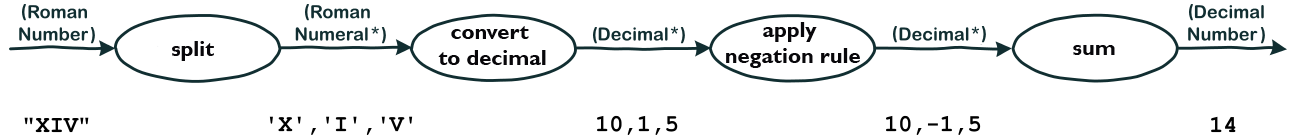
\includegraphics[width=1.0\linewidth]{./img/FromRomanNumerals.png}
	\caption{Einfaches Flow Design Beispiel}
\end{figure}
\end{center}




Das Beispiel soll auf einfache Weise zeigen, wie ein Flow Design Diagramm aufgebaut ist.
Das Programm/Unterprogramm soll eine römische Zahl in eine Dezimalzahl konvertieren.

Alle eingekreisten Namen sind Funktionseinheiten.
Diese werden in den meisten Fällen im Code als Methoden implementiert.
Die Pfeile zeigen den Datenstrom. Links die Inputs und rechts die Outputs.


Der Input-Datenstrom der ersten Funktionseinheit besteht aus einem String. Dieser String wird zerlegt in einzelne Buchstaben.
Der Buchstabenstrom fließt anschließend in eine weitere Funktionseinheit, die jeden Buchstaben zu der entsprechenden
Dezimalzahl konvertiert. Anschließend muss auf den Strom noch die Subtraktionsregel angewendet werden. Diese untersucht den
Strom aus Ganzzahlen auf Stellen, wo eine kleinere Zahl vor einer größeren Zahl steht und sie in dem Fall dann negativ macht.
Am Ende wird der Datenstrom einer Funktionseinheit übergeben, die alle Zahlen aufaddiert.
Das Ergebnis ist die Summe aller Zahlen.


\newcommand\blfootnote[1]{%
	\begingroup
	\renewcommand\thefootnote{}\footnote{#1}%
	\addtocounter{footnote}{-1}%
	\endgroup
}

\chapter{Die Notation}

\section{Datenströme}

 \blfootnote{Die meisten der Bilder in diesem Kapitel stammen von \cite{flowdesignorg}}
 
\begin{figure}[H]
	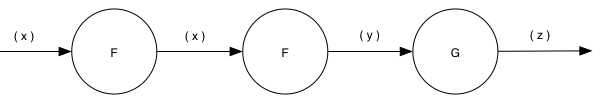
\includegraphics[width=1\linewidth]{./img/diagram1.png}
	\caption{Datenfluss zwischen drei Funktionseinheiten}
\end{figure}






Über den Pfeilen, die die Richtung des Datenflüssen darstellt, werden die im
Datenfluss enthaltenen Datentypen in runden Klammern eingetragen.

Eine leere Klammer bedeutet, dass ein Datenstrom ohne Daten fließt.
Die Funktionseinheit wird einfach nur aufgerufen, ohne ihr Daten zu übergeben.


Die Notation erlaubt es auch einzelne Datentypen zusätzlich noch mit einem Namen
zu versehen. Was vor allem bei primitiven Datentypen hilfreich sein kann. 
Der optionale Namen wird dem Datentyp durch einen Doppelpunkt getrennt vorangestellt.

\begin{figure}[H]
	\centering
	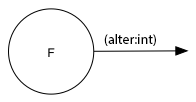
\includegraphics[width=.4\linewidth]{./img/diagramNamedType.png}
	\caption{Datentyp \textit{int} mit Namen \textit{alter}}
\end{figure}


Falls der Datentyp aus dem Namen hervorgeht - oder nicht allzu relevant ist - kann auch anstatt des Datentypen nur der Namen in die runden Klammern eingetragen werden.


\clearpage

\section{Hierarchische Datenflüsse}



\begin{figure}[H]
	\centering
	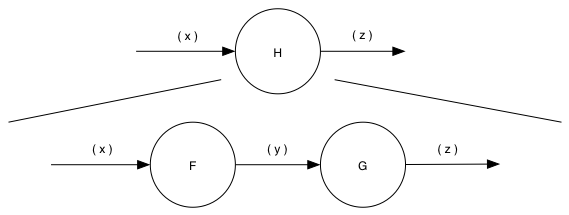
\includegraphics[width=1\linewidth]{./img/diagramHir.png}
	\caption{Hierarchischer Datenfluss}
\end{figure}


Das Flow Design Flussdiagramm unterstützt die Funktion in eine Funktionseinheit sozusagen hineinzuzoomen.
Hier erkennt man die rekursive Eigenschaft der Funktionseinheiten:
Eine Funktionseinheit kann wiederum aus mehreren Funktionseinheiten bestehen,
die zusammen die Aufgabe erledigen, die die übergeordnete Funktionseinheit
beschreibt. Eine solche übergeordnete Funktionseinheit wird als Integration
bezeichnet. Hat eine Funktionseinheit keine untergeordneten Funktionseinheiten wird sie
als Operation bezeichnet. Was es mit dieser Aufteilung genau auf sich hat, wird im
Kaptiel 4 erläutert.


\section{Definition eigener Datentypen}






\begin{figure}[H]
	\centering
	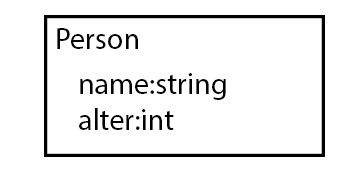
\includegraphics[width=.35\linewidth]{./img/diagramCustomTypes.png}
	\caption{Eigener Datentype}
\end{figure}


Bei einen Datenstrom bestehend aus einem eigenen Datentypen, kann es helfen, den Datentyp innerhalb des Flow Design Diagrammes zu definieren.
Dafür wird an einer beliebigen Stelle auf dem Papier eine Box gezeichnet,
in der der Datentyp mit seinen Membervariablen aufgelistet wird.\footnote{Diese Notation ist nicht offiziell Teil der Flow Design Notation,
sondern ist eine Ergänzung von Kevin Erath}

\section{Arrays}

\begin{figure}[H]
	\centering
		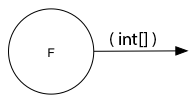
\includegraphics[width=.5\linewidth]{./img/diagramArray.png}
	\caption{Array Notation}
\end{figure}

Werden Daten als Arrays mit fester Größe übergeben, so wird hinter dem Datentyp eine leere eckige Klammer angehängt.
Ist die Arraygröße bekannt, so kann man diese in die Klammer noch zusätzlich eintragen.



\section{0 bis n (Datenstrom)}


\begin{figure}[H]
	\centering
	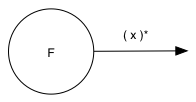
\includegraphics[width=.5\linewidth]{./img/diagram0n.png}
	\caption{Datenstrom Notation}
\end{figure}



Ein Datenstrom wird mit einem * außerhalb der Klammer dargestellt.
Selten wird ein Datenstrom auch mit geschweiften Klammern dargestellt, um ihn
von einem optionalen Output ( 0 bis 1 ) unterscheiden zu können: \{int\}.

Ein Datenstrom zeigt an, dass die in der Klammer stehenden Daten keinmal,
einmal, oder auch öfters als einmal fließen können.

\section{Container / Listen}


\begin{figure}[H]
	\centering
	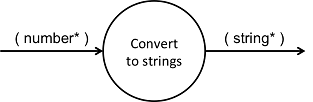
\includegraphics[width=.7\linewidth]{./img/diagramCollection.png}
	\caption{Container Notation}
\end{figure}


Stern innerhalb der Klammer.
Der Datentyp liegt in einem Container vor.
Die zu bearbeitende Daten können entweder komplett auf einmal an die Funktionseinheit gegeben werden ( als Liste, Dictionary, etc. )
oder aber - falls die Programmiersprache dies unterstützt - als yield ähnlich
wie ein Stream realisiert werden, wo einzelne Elemente bereits abgearbeitet werden
können, bevor alle anderen Daten erzeugt wurden.

\section{0 bis 1 (optionaler Output)}

\begin{figure}[H]
	\centering
	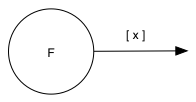
\includegraphics[width=.5\linewidth]{./img/diagramOptional.png}
	\caption{Optionaler Output}
\end{figure}


Mit einer eckigen Klammer lässt sich ein optional Output - einmal oder keinmal -
darstellen. \footnote{Oft wird jedoch auf diese Notation verzichtet und auch bei optionalen Ausgängen eine runde Klammer verwendet. 
}

Optionale Outputs können genau wie Datenströme nicht über ein Rückgabewert einer
Methode realisiert werden, da nach jedem Aufruf genau ein Rückgabewert erwartet wird. Wie solche
Datenflüsse in C\# realisiert werden, wird in einem späteren Kapitel gezeigt.

\section{Mehrere Datentypen auf einem Datenstrom}


\begin{figure}[H]
	\centering
	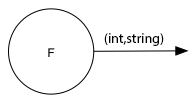
\includegraphics[width=.5\linewidth]{./img/diagramIntString.png}
	\caption{Mehrere unterschiedliche Datentypen auf einem Datenstrom}
\end{figure}


Besteht ein Datenstrom einer Funktionseinheit aus mehrere Datentypen, so werden diese durch Kommas getrennt in die Klammer geschrieben.

Mehrere Outputs lassen sich nicht in allen Sprachen einfach realisieren.
Wahlweise kann es mit Tupel realisiert werden, oder es werden aus den mehreren Datentypen ein 
neuer Datentyp erzeugt, der alle Output-Daten beinhaltet.

\section{Joined Inputs und Pipe-Notation}

\begin{figure}[H]
	\centering
	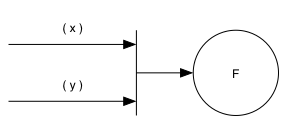
\includegraphics[width=.7\linewidth]{./img/diagramJoin.png}
	\caption{Joined Inputs}
\end{figure}


Falls der Output mehrere Funktionseinheiten in einen Datenstrom zusammenlaufen
sollen und dieser dann als Input in eine anderen Funktionseinheit hineinfließen
soll, wird das mit Hilfe eines s.g. Joined Inputs dargestellt. 
Dieser wird als Linie dargestellt an die mehrere Inputs zusammenlaufen.

Im Code wird dies meistens als Methode umgesetzt, die mehrere Inputparameter entgegennimmt.
Wichtig hierbei ist, dass das Bündeln der Datenflüsse nicht Aufgabe der
Funktionseinheit \textit{F} ist, sondern ihrer Umgebung ( z.B einer übergeordneten Methode).
Die Funktionseinheit \textit{F} erwartet einfach ein Datenstrom mit zwei Daten \textit{x} und \textit{y}
und kennt deren Herkunft nicht.

\bigskip
Eine andere Schreibweise, die im Diagramm platzsparender ist als die Joined Inputs, ist die Pipe-Notation.
Hiermit kann der Output sich von dem Input der nachfolgenden Funktionseinheit unterscheiden.
Dadurch können auch Daten, die aus vorherigen Funktionseinheiten innerhalb des Datenflusses entstanden sind, entnommen und einer Funktionseinheit
übergeben werden.

\begin{figure}[H]
	\centering
	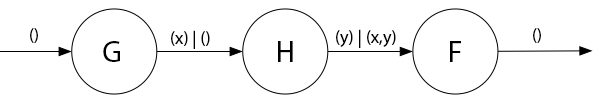
\includegraphics[width=\linewidth]{./img/diagramPipe.jpg}
	\caption{Pipe-Notation}
\end{figure}

In diesem Beispiel produziert \textit{G} ein \textit{x} und \textit{H} ein \textit{y}. Sowohl \textit{G} als auch \textit{H} nehmen keine Daten beim Aufruf entgegen.
In die Funktionseinheit \textit{F} fließen die Daten aus \textit{G} und \textit{H} zusammen.

\section{Tonnen}

\begin{figure}[H]
	\centering
		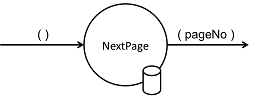
\includegraphics[width=.7\linewidth]{./img/diagramTonne.png}
	\caption{Tonnensymbol}
\end{figure}



Eine Tonne zeigt an, dass die Funktionseinheit state-behaftet ist.
In einer OO-Sprache wie C\# wäre das in den meisten Fällen ein Lesen oder
Schreiben einer Membervariable einer Klasse.

\section{Abhängigkeiten / Provider}

\begin{figure}[H]
	\centering
		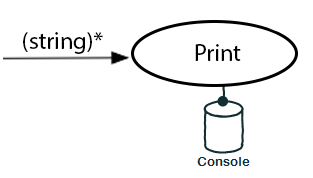
\includegraphics[width=.5\linewidth]{./img/diagramProvider.png}
	\caption{Provider}
\end{figure}



Eine Tonne die mit einer Linie zu einer Funktionseinheit verbunden ist, soll
anzeigen, dass die Funktion auf externe Ressourcen zugreift, wie zum
Beispiel eine Datei oder Datenbank. 
Geschieht der Zugriff auf die Ressource über eine Helferklasse, die den Zugriff
kapselt, wird anstelle der Tonne ein Dreieck als Symbol verwendet. Eine solche
Klasse wird auch als Provider bezeichnet. 

Den Kreis kann man sich bildlich wie eine Hand vorstellen, an die sich die
Funktionseinheit festhält, und dadurch eine Abhängigkeit symbolisiert.

\pagebreak

\section{GUIS / Programmstart/ Ende}

\begin{figure}[H]
	\centering
		
\includegraphics[width=.9\linewidth]{./img/diagramStartEnd.png}
	\caption{Programmstart und Programmende}
\end{figure}




Wenn eine Funktionseinheit direkt durch den Programmstart aufgerufen wird, so
wird dies mit einem leeren Kreis dargestellt. Genau so verhält es sich mit dem
Programmende, mit der Unterschied, dass noch innerhalb des Kreises ein Kreuz ist.

\begin{figure}[H]
	\centering
		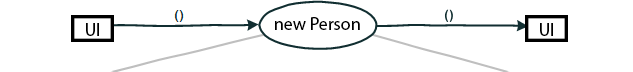
\includegraphics[width=.9\linewidth]{./img/diagramUI.png}
	\caption{UI}
\end{figure}


Soll dargestellt werden, dass eine Funktionseinheit von einem Event aus der GUI ausgelöst
wurde, oder die ausgehenden Daten einer Funktionseinheit in das GUI übergeben werden, so
wird ein Viereck am Anfang bzw. Ende des Pfeiles eingezeichnet.

\section{Klassen / Container definieren}


\begin{figure}[H]
	\centering
	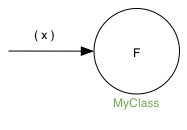
\includegraphics[width=.4\linewidth]{./img/diagramClass.png}
	\caption{Zugehörigkeit zu einer Klasse}
\end{figure}


Das Definieren von Container und Zuordnen von Funktionseinheiten ist auch
einfach möglich. Unter Container versteht man: Klassen, DLLs und Anwendungen.
Es gibt zwei Möglichkeiten eine Zugehörigkeit zu einem Container zu notieren.
Entweder man schreibt direkt unter der Funktionseinheit den Namen des
Containers, oder man umrandet mehrere Funktionseinheiten und notiert den Namen
des Containers am Rand der Umrandung.

%TODO wohin mit dieser Anmerkung?

\blankfootnote{Bilder sind von:
\url{http://flow-design.org/overview/implementation/\#How_to_implement_inputs_to_a_functional_unit}}

\chapter{Implementation}


Flow Design hat 2 Implementierungsregeln, die zu beachten sind:

\begin{itemize}
\item Trennen von Integrationen und Operationen
\item keine funktionale Abhängigkeiten in Operationen zu anderen Funktionseinheiten aus dem selben Programm
\end{itemize}

Um was es sich dabei im Detail genau handelt, wird in diesem Kapitel erläutert.

\pagebreak
\section{IODA Architektur}

\abk{IODA}{Integration Operation Data API}

Wie schon in dem vorherigen Kapitel angemerkt, unterscheidet Flow Design zwei
unterschiedliche Arten von Funktionseinheiten. Integrationen und Operationen.
Die IODA Architektur beschreibt die Eigenschaften von diesen beiden genauer.

IODA steht für: Integration Operation Data API


\begin{figure}[H]
	\centering
	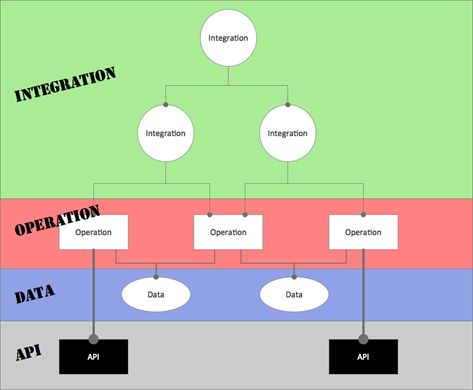
\includegraphics[width=.9\linewidth]{./img/ioda1.png}
	\caption{IODA Architektur}
\end{figure}



\let\thefootnote\relax\footnotetext{\url{http://blog.ralfw.de/2015/04/die-ioda-architektur.html}}
\subsubsection{Erläuterung des Schaubildes}

Operationen sollen komplett unabhängig vom Rest ihrer Umwelt funktionieren und
dürfen aus diesem Grund andere Funktionseinheiten nicht kennen.

Die Aufgabe einer Integration ist, die unabhängigen Operationen in das große Ganze zu
Integrieren. 
(Fußnote) Ralf Westphal spielte auch mit den Gedanken diese Funktionseinheiten als Koordinatoren oder
Kompositionen zu bezeichnen.

Integrationen integrieren andere Integrationen und/oder Operationen in das Programm. Sie dürfen also funktional abhängig sein
von anderen von Funktionseinheiten.

Im Gegensatz dazu dürfen Operationen keine Integrationen oder andere Operationen
kennen. Sie dürfen aber auf Daten zugreifen. Über diese entsteht auch die einzige Möglichkeit der
Kommunikation zwischen Operationen. Mit Daten sind hauptsächlich die inpersitente
Daten gemeint. Daten in Form von Objekten und primitive Datentypen, die von den
integrierenden Funktionseinheiten koordiniert werden.
Sowohl Operationen als auch Integrationen dürfen Daten Erzeugen.
Beispielsweise das Aufrufen eines Konstruktors oder Deklarieren einer lokalen Variablen.
Das "Verdrahten" von Datenflüssen übernehmen jedoch die Integrationen ( was auf
dem Schaubild leider nicht so deutlich herauskommt). 
Mit Daten können auch persistente Daten auf der Festplatte gemeint sein, wobei
ein Zugriff auf persistente Daten eigentlich immer über eine API geschieht und
somit würden solche Aufrufe dann eher zu der Gruppe API zählen.

Die IODA Architektur besagt, dass API-Aufrufe sich nur innerhalb von Operationen befinden
dürfen, damit diese Informationen gekapselt und die Integrationen frei von API-spezifisches Wissen bleiben.


Anhand einer Flow Design Skizze, kann man leicht herausfinden, welche Methoden Operationen sind und welche
Integrationen. Alle Leaf-Knoten sind Operationen, der Rest sind Integrationen.


\subsubsection{PoMO ( Principle of Mutual Oblivion)}

\abk{PoMO}{Principle of Mutual Oblivion}

\def\signed #1{{\leavevmode\unskip\nobreak\hfil\penalty50\hskip2em
		\hbox{}\nobreak\hfil(#1)%
		\parfillskip=0pt \finalhyphendemerits=0 \endgraf}}

\newsavebox\mybox
\newenvironment{aquote}[1]
{\savebox\mybox{#1}\begin{quote}}
	{\signed{\usebox\mybox}\end{quote}}

\begin{aquote}{Ralf Westphal \cite[S. 80]{schummelzettel}}
	Ein Producer kennt seinen Consumer nicht. Ein Consumer kennt seinen Producer
	nicht. Das nenne ich das Principle of Mutual Oblivion (PoMO,
	Prinzip der gegenseitigen Nichtbeachtung) 
\end{aquote}




Dieses Prinzip besagt, dass Funktionseinheiten sich nicht gegenseitig kennen sollen.
Es soll auch verhindert werden, dass eine Einheit eine andere aufruft und von deren Ergebnis
abhängig ist, bzw. auf das Ergebnis wartet.
Eine Funktionseinheit soll, nachdem sie die Daten bearbeitet hat, sie einfach nach
außen weiter reichen und nicht wissen, wer die Daten entgegennimmt.
Dieses Prinzip verhindert eine Koppelung zwischen den einzelnen Funktionseinheiten.

Um jedoch ein Zusammenspiel zwischen den einzelnen entkoppelten Einheiten zu ermöglichen, bedarf es einen oder
mehrere "Koordinatoren" welche diesem Prinzip nicht entsprechen müssen.
Nur so kann aus vielen kleinen Funktionseinheiten ein großes Ganzes werden, dass eine komplexe Aufgabe lösen kann.
Damit die das Zusammenspiel leicht zu modifizieren bleibt und die Verdrahtung
leicht zu verstehen sind gelten für Integrationen einige Einschränkungen, die
unter der Namen "Integration Operationen Segregation Principle" zusammengefasst
werden.



\subsubsection{IOSP ( Integration Operation Segregation Principle)}

\abk{IOSP}{Integration Operation Segregation Principle}

Dieses Prinzip besagt, dass eine Funktionseinheit entweder eine Operation oder eine Integration ist und beide
Verantwortungsbereiche nicht vermischt werden dürfen.

\begin{enumerate}
\item Operationen




Operationen sind Methoden, die Logik/ Kontrollstrukturen enthalten dürfen. In C\# wären das:
\begin{itemize}
\item if, else
\item switch, case
\item for, foreach,
\item while, do
\item try, catch, finally
\item goto
\end{itemize}




Gleichzeitig müssen die Operationen das PoMO Prinzip erfüllen, sie dürfen nicht
wissen, er die Daten bekommt oder was damit passiert, aus diesem Grund darf auch
kein Rückgabewert erwartet werden, sonst lassen sich daraus Rückschlüsse bzw. Erwartungen verknüpfen.
Ein Funktionsaufruf ist nur über Actions ( Funktionszeiger ), die man als Funktionsparameter mit übergibt, oder Events möglich.
Beide dürfen keine Rückgabewerte haben, was bei Actions implizit der Fall ist.
Durch diese Regel wird einer Operation ermöglicht eine andere Funktion
aufzurufen, ohne das sie das PoMO bricht. Sie bestimmt nicht selbst, welche
Funktion sie aufruft, sondern die übergeordnete Funktion, welche die Operation
aufruft ( und somit automatisch eine Integration sein muss, welche die PoMO Bedingung nicht erfüllen muss).
Wie das praktisch aussieht, wird im Laufe des Kapitels anhand von konkreten
Beispiel genauer veranschaulicht.

Operationen sind also imperative programmiert. Imperative Programmierung ist ein Programmierstil,
mit dem Fokus auf das \textbf{wie} ein Problem gelöst werden soll.
Im Gegensatz dazu steht der deklarative Ansatz.
Beim deklarativen Programmieren steht der Fokus auf das \textbf{was} getan werden soll und nicht so sehr,
wie es im Detail genau angestellt wird. Ein Beispiel hierfür wären zum Beispiel SQL Befehle.
Hier wird nur gesagt, was man haben möchte und das Programm kann dann die Anfrage nochmal untersuchen
und selbst bestimmen, wie es die Anfrage am besten ausführt.

\item Integrationen


Die Integrationen werden nach Flow Design deklarative programmiert.
Diese Funktionseinheiten dürfen anders als die Operationen, andere Funktionseinheiten aufrufen, sie also kennen.
Die Integrationen erfüllen also nicht das \emph{Principle of Mutual Oblivion}
Der Unterschied beim Flow Design ist jedoch, dass eine bewusste Trennung eingehalten wird.

Integrationen dürfen auch auf die Terminierung einer Funktionseinheit warten und den Rückgabewert  weiterreichen an andere Funktionseinheiten.
Dafür dürfen sie keine Logik im Sinne von Kontrollstrukturen beinhalten.
Auch dürfen sie keine API-spezifischen Befehle kennen, wie zum Beispiel Zugriffe
auf Ressourcen wie Konsole, UI oder Dateien.

Die Businesslogik, das was die Funktionalität erzeugt, diese befinden sich in Operationen und sind entkoppelt von ihrer Umgebung.
Sie bekommen einfach nur von irgendwo her einen Input (bzw. bei keinen Inputparametern einfach ausgeführt werden) und führen damit die von ihnen implementierte
Logik aus und geben das Ergebnis nach außen. Beim nach außen Reichen kennt die Funktionseinheit jedoch nicht den Empfänger.
\end{enumerate}

\subsubsection{Tabelle -  IOSP auf einen Blick}


\bigskip
\begin{table}[H]
	\centering
\begin{tabularx}{\textwidth}{|X|l|l|}
	\hline
 & Operationen & Integrationen\\
\hline
Rechenoperationen ( +, *, \%, \ldots{} ) & Ja & Nein\\ \hline
Kontrollstrukturen (if, else, while, for, foreach, \ldots{}) & Ja & Nein\\ \hline
API-Aufrufe (Methoden von Bibliotheken) & Ja & Nein\\ \hline
Ressourcen-Zugriffe (Dateien, Datenbanken etc.) & Ja & Nein\\ \hline
Standard Library, LINQ & Ja & Ja\\ \hline
Namen andere Funktionseinheiten kennen & Nein & Ja\\ \hline
Auf Rückgabewert warten & Nein & Ja\\ \hline
\end{tabularx}
	\medskip
	\caption{IOSP Übersicht}
\end{table}



\section{Beispiel foreach und Funktionsaufruf}




\begin{lstlisting}[caption=FormatAndPrintStrings nicht IOSP-konfrom]
static void FormatAndPrintStrings(List<string> lines)
{
   foreach(line in lines)
   {
      string s = MyComplexFormattingFunction(line);
      Console.WriteLine(s);
   }
}
\end{lstlisting}
Derartiger Code wird wohl in den meisten C\#-Codebasen zu finden sein und doch ist er nach Flow Design falsch.

In diesem Beispiel wurde Logik (foreach) gemischt mit einem expliziten
Methodenaufruf, sowie ein Zugriff auf eine externe Ressource, die
Konsole.

Diese Methode ist somit nicht IOSP konform.

Es ist etwas ungewohnt, das Trennen von Integrationen und Operationen im Code auch zu berücksichtigen.
Eine For-Schleife über eine Kollektion laufen zu lassen und jedes Element an eine Untermethoden weiterzureichen ist etwas,
was wohl viele Programmierer regelmäßig so schreiben.
Das so etwas nun nicht mehr erlaubt ist, braucht eine gewissen Umgewöhnungszeit.

\bigskip

Hier nun die Umsetzung in Flow Design mit einfachsten Mitteln:

\begin{lstlisting}[caption=FormatAndPrintStrings Variante 1]
// Integration
static void FormatAndPrintStrings(List<string> lines)
{
   List<string> formattedLines = FormatLines(lines);
   PrintLines(formattedLines);
}

// Operationen
static List<string> FormatLines(List<string> lines)
{
    List<string> result = new List<string>();
    foreach(line in lines)
    {
          string formattedstring;
          // do complex formatting here
          result.Add(formattedstring)
    }
    return result;
}

static void PrintLines(List<string> lines)
{
   foreach(line in lines)
   {
      Console.WriteLine(line);
   }
}
\end{lstlisting}


Als Flow Design dargestellt, würde der Code folgendermaßen aussehen:
\begin{figure}[H]
	\centering
	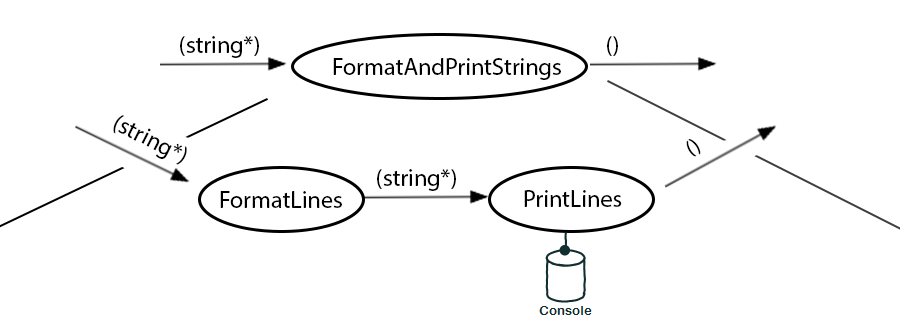
\includegraphics[width=1\linewidth]{./img/flowForeach1.png}
	\caption{FormatAndPrintStrings Variante 1 - Flow Design}
\end{figure}


Die Methode wurde aufgeteilt in eine Integration (\texttt{FormatAndPrintStrings}) und zwei Operationen.
Im ersten Beispiel hat die Methode zwei Aufgaben erfüllt, sie hat die Formatierung-Methode integriert und
das Ergebnis ausgegeben.

Nun sind Integration, Ausgabe und Formatierung sauber getrennt. Womit das SRP
auch erfüllt ist. Womit das SRP auch erfüllt ist. Dadurch wurde eine Entkopplung geschaffen, 
die Änderungen am Code leichter macht. Besonders vorteilhaft, das UI ist getrennt vom Rest

Jedoch wurde der Code nun deutlich länger. Die Foreach-Schleife ist in beide Operationen gelandet und das Initialisieren und
Befüllen der temporären Liste in \texttt{FormatLines} nimmt auch etwas Platz ein.
Dazu kommt noch, das die String-Formattierungslogik nun eingebettet in dieser Foreach-Schleife liegt, welche sich vorher getrennt in
einer extra Methode  befand.

\bigskip

Elegantere Lösung mit Actions:

\begin{lstlisting}[caption=FormatAndPrintStrings Variante 2]
// Integrationen
static void FormatAndPrintStrings(List<string> lines)
{
   IterateOverLines(lines, onLine=PrintFormat );
}

static void FormatAndPrint(string line)
{
   var formattedline = MyComplexFormattingFunction(line);
   Print(formattedline);
}

// Operationen
static void IterateOverLines(IEnumerable<string> lines, Action<string> onLine)
{
   foreach(line in lines)
   {
      onLine(line);
   }
}

static void Print(string line)
{
   Console.WriteLine(line);
}


\end{lstlisting}

Als Flow Design dargestellt, würde der Code folgendermaßen aussehen:

\begin{figure}[H]
	\centering
	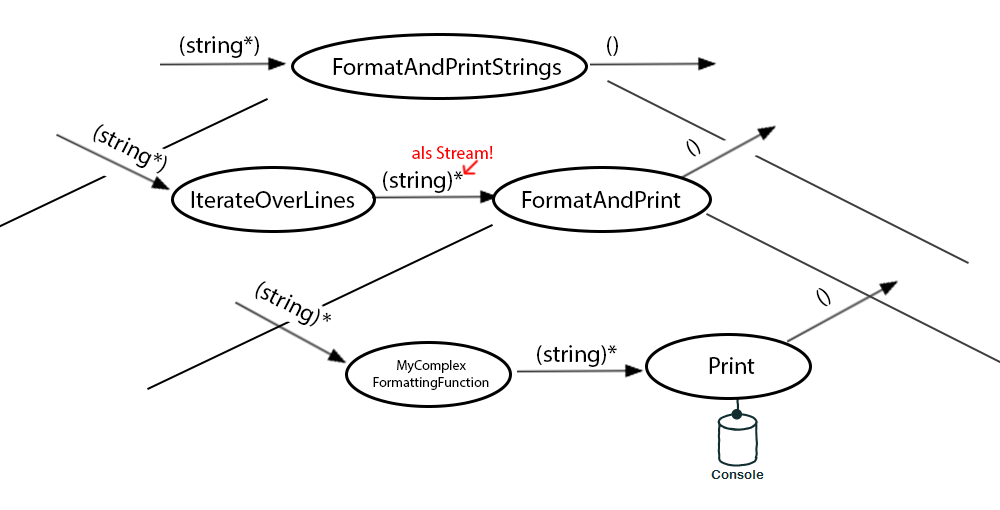
\includegraphics[width=1\linewidth]{./img/FlowsForeach.png}
	\caption{FormatAndPrintStrings Variante 2 - Flow Design}
\end{figure}



Noch eleganter mit Actions und Lambdas:

\begin{lstlisting}[caption=FormatAndPrintStrings Variante 3]
static void FormatAndPrintStrings(List<string> lines)
{
  IterateOverLines(lines,
    line => {
      var formattedline  = MyComplexFormattingFunction(line);
      Print(formattedline);
  });
}

static void IterateOverLines(IEnumerable<string> lines, Action<string> onLine)
{
   foreach(line in lines)
   {
      onLine(line);
   }
}

static void Print(string line)
{
    Console.WriteLine(line);
}
\end{lstlisting}


Eine weitere Möglichkeit besteht darin Datenfluss orientierte Sprachfeatures zu verwenden.
Somit hängt diese Möglichkeit stark von der verwendetet Programmiersprache ab.
In C\# existiert eine Kategorie an Methoden, die speziell auf das Arbeiten mit Datenflüssen ausgerichtet ist, diese werden
zusammengefasst unter dem Namen LINQ (Language-Integrated Query).
\abk{LINQ}{Language-Integrated Query}

\bigskip
Mit Hilfe von LINQ lässt sich obiges Beispiel zu einem IOSP konformen Einzeiler reduzieren.

\begin{lstlisting}[caption=FormatAndPrintStrings Variante LINQ]
static void FormatAndPrintStrings(List<string> lines)
{
   lines.Select( x => MyComplexFormattingFunction(x)).ToList()
	   .ForEach(Console.WriteLine);
}
\end{lstlisting}

Man könnte sich nun darüber streiten, was man nun damit gewonnen hat. Schließlich enthält die Funktion mit LINQ im Grunde
genommen fast nun genau die selbe Logik, wie das nicht IOSP-konforme Beispiel, nur mit einer anderen Schreibweise.
Der Nutzen dieser Regel erschließt sich erst, bei größeren Codebasen und kommt bei kleinen Beispielen oft nicht zum Vorschein.
Erst wenn die Integrationen mehr machen, als nur eine Funktion aufrufen, wird das Entkoppeln nützlich.
Außerdem ist der Fall einer Foreach-Schleife und ein Funktionsaufruf eine Koppelung, die nicht so dramatisch ist. Man
könnte für diesen Fall sogar eine Ausnahme machen und sie erlauben.


Zusammenfassend könnte noch gesagt werden, dass eine größere Lesbarkeit von IOSP konformen Programmcode entsteht, umso mehr moderne und funktionale
Sprachfeatures eine Programmiersprache bietet.

\section{C\# Features um Datenflüsse zu implementieren}

Um Flow Design gemäß der IODA Architektur umzusetzen, helfen einem in C\# einige Features die in diesem Kapitel vorgestellt werden.

\subsubsection{LINQ und Lambdas}

Streng genommen würde es die IODA Architektur nicht erlauben die Methoden der
Standardbibliothek innerhalb von Operationen zu verwenden. Jedoch würde das den
Code nur unnötig verkomplizieren ohne wirklich ein Nutzen daraus zu gewinnen.
Aus diesem Grund ist es sinnvoll die Methoden der Standardbibliothek der Sprache
in Operationen als auch in Integrationen zu erlauben.
In C\# gehört dazu auch die Methodensammlung LINQ. 
LINQ ist eine in C\# integrierte Ansammlung an Methoden die in Verbindung mit
Objekten, die das IEnumerable Interface implementieren, eingesetzt werden
können.
IEnumerable ist das Interface einer Aufzählungsklasse. Daran lässt sich bereits erahnen, dass LINQ
auf das Arbeiten mit Datenflüssen spezialisiert ist.

In den meisten Fällen werden den LINQ Methoden ein Lambda-Ausdruck übergeben.
Dieser wird auch als \texttt{Selector} bezeichnet, oder im Falle von Bedingungen als \texttt{Predicate}.
Lambda-Ausdrücke werden nach Flow Design Regeln, wie eigenständige
Funktionseinheiten betrachtet. Somit darf ein Lambda innerhalb einer 
Integrationen auch eine Operation sein.


\blankfootnote{LINQ besteht aus ca. 150 Methoden.
	Eine (nicht vollständige Liste) befindet sich hier: \url{https://msdn.microsoft.com/en-us/library/system.linq.enumerable_methods}} 


\bigskip
Im Folgendem werden hier nur ein paar der häufigsten verwendeten Methoden erläutert.

\begin{enumerate}
\item Modifizieren

Folgende Methoden verändern den Datenstrom und liefern einen neuen Datenstrom
zurück (mit Ausnahme von ForEach).

\bigskip
\begin{table}[H]
	\centering
\begin{tabularx}{\textwidth}{|p{130 pt}|X|}
		\hline
Select & Selektiert jedes Element und der Sequenz und modifiziert es. Zurückgegeben wird eine Sequenz der modifizierten Elemente\\	\hline
ForEach (nur für List-Klasse) & Iteriert über die Sequenz und führt mit jedem Element den Selector-Ausdruck aus. Im Gegensatz zu Select wird kein Sequenz zurückgeliefert. Diese Methode ist nicht Teil von LINQ sondern gehört ausschließlich zu der List-Klasse. Da sie jedoch oft Verwendung findet in LINQ-Ausdrücke, wird sie hier mit aufgezählt\\	\hline
First,  Last & Gibt das erste/letzte Element der Sequenz zurück, das eine bestimmte Bedingung erfüllt.\\	\hline
OrderBy & Ordnet die Sequenz mit Hilfe eines \texttt{keySelector}-Ausdrucks. Dieser bestimmt das Sortierkriterium. In manchen Fällen (Elemente sind Zahlenwerte, oder Strings), kann dieser weggelassen werden, falls das Default-Verhalten gewünscht ist\\	\hline
Distinct & Duplikate werden aus der Sequenz gelöst.\\	\hline
Join & Zwei Sequenzen werden zu einer zusammengefasst\\	\hline
\end{tabularx}
	\medskip
	\caption{LINQ - Sequenzen Modifizieren}
\end{table}


\item Filtern

\bigskip

\begin{table}[H]
	\centering
\begin{tabularx}{\textwidth}{|p{130 pt}|X|}
		\hline
Where & Filtern der Sequenz anhand des Predicate. Zurückgegeben wird eine Sequenz von Elementen, die das Filterkriterium entsprachen.\\	\hline
\end{tabularx}
	\medskip
	\caption{LINQ - Sequenzen Filtern}
\end{table}

\item Überprüfungen

Diese Methoden liefern einen Boolean als Rückgabewert zurück.

\bigskip
\begin{table}[H]
	\centering
\begin{tabularx}{\textwidth}{|p{130 pt}|X|}
		\hline
Any & Wendet auf jedes Element den Selector-Ausdruck solange an, bis bei einem Element der Ausdruck wahr wird. Dann wird \texttt{true} zurückgegeben, ansonsten \texttt{false}\\	\hline
Contains & Ähnlich wie \texttt{Any}, nur dass kein Selector übergeben wird, sondern ein Element, der selben Klasse, wie die Elemente des Containers. Befindet sich das Element in dem Container, dann wird \texttt{true} zurückgeben, ansonsten \texttt{false}\\	\hline
All & Ähnlich wie \texttt{Any} mit dem Unterschied, dass nur dann \texttt{true} zurückgeben wird, wenn für alle Elemente des Containers der Ausdruck wahr ist.\\	\hline
\end{tabularx}
	\medskip
	\caption{LINQ - Sequenzen Überprüfen}
\end{table}

\item Berechnungen

Bei Container mit Zahlenwerten (\texttt{int}, \texttt{float}, \texttt{decimal},\ldots{}) als Elementen,
können nachfolgende Funktionen ohne zusätzliche Parameter aufgerufen werden.
Falls dies nicht der Fall ist, muss ein Selector-Ausdruck, wahlweise als
Lambda-Ausdruck, mit übergeben werden. Mit dem Selector kann bestimmt werden, wie
die mathematische Rechenoperationen mit jedem Element umzugehen hat.

\bigskip
\begin{table}[H]
	\centering
\begin{tabularx}{\textwidth}{|p{130pt}|X|}
	\hline
Sum & Aufsummieren der Elemente\\ 	\hline
Max & Gibt das Element mit dem höchsten Wert zurück\\	\hline
Min & Gibt das Element mit dem niedrigsten Wert zurück\\ 	\hline
Count & Zählt die Elemente des Containers und gibt die Anzahl zurück\\	\hline
Average & Berechnet den Durchschnitt der Sequenz\\	\hline
\end{tabularx}
	\medskip
	\caption{LINQ - Berechnungen}
\end{table}

\item Überspringen und Nehmen

Diese Methoden liefern genau wie die modifizierenden Methoden als Rückgabewert
eine neue Sequenz an Daten zurück.

\bigskip
\begin{table}[H]
	\centering
\begin{tabularx}{\textwidth}{|p{130pt}|X|}
	\hline
TakeWhile & Nimmt Elemente solange aus dem Container, bis eine Bedingung erfüllt ist. Es wird eine Sequenz von allen genommenen Elementen zurückgegeben\\	\hline
Skip & Überspringt eine Anzahl an Elementen\\	\hline
SkipWhile & Überspringt die ersten Elemente einer Sequenz, solange bis die Bedingung von einem Element nicht erfüllt wird, dann wird ohne weitere Überprüfungen der Rest der Sequenz zurückgegeben\\	\hline
\end{tabularx}
	\medskip
	\caption{LINQ - Überspringen und Nehmen}
	
\end{table}

\item Konvertieren

Sequenzen können mit Hilfe eines einfachen Methodenaufrufs zu einem bestimmten Typ
von Container konvertiert werden. Zum Beispiel: \texttt{ToList} oder \texttt{ToDictionary}.

\item Parallele Verarbeitung

Datenströme können von LINQ auch parallel verarbeitet werden. Dazu konvertiert
man die Sequenz mit \texttt{toParallel()} zu einem PLINQ Datenstrom.
Anschließend ausgeführte Methoden werden, falls möglich parallel verarbeitet.

\end{enumerate}

\blankfootnote{Quelle: \url{https://www.dotnetperls.com/linq}} 

\subsubsection{yield return}

Hiermit kann man ein Producer-Consumer Pattern implementieren.
Voraussetzung ist hierfür, dass der Rückgabewert der Methode ein \texttt{IEnumerable} Interface ist.

Das folgende Flow Design soll mit \texttt{yield return} realisiert werden.

\begin{figure}[H]
	\centering
	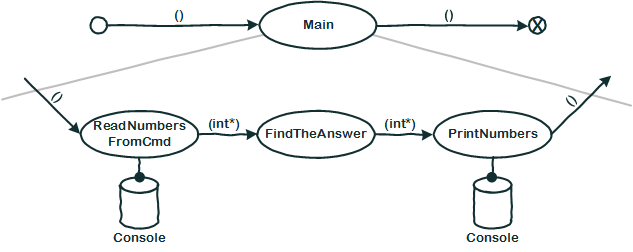
\includegraphics[width=\linewidth]{./img/FlowDesign2.png}
	\caption{FindTheAnswer - Flow Design}
\end{figure}



\blankfootnote{\url{http://www.code-whisperer.de/preview/2015/06/14/eva/}}

\bigskip
Das Programm ist eine Konsolenanwendung, die dem Benutzer eine Eingabe erlaubt.
Wenn die Eingabe die Zahl 42 entspricht, wird das Programm beendet, wenn nicht,
dann wird die Zahl ausgegeben und der Benutzer kann wieder eine Zahl eingeben.
Das wiederholt sich, solange bis der Benutzer die Zahl 42 eingetippt hat.


\begin{enumerate}
\item Erläuterung des Schaubildes

Die  Main-Methode wird nach dem Programmstart ( leerer Kreis ) ohne Parameter aufgerufen.
Danach ruft diese die Methode \\\texttt{ReadNumbersFromCmd} auf, welche aus der Konsole eine Eingabe ließt und sie
zu einem int parset. Der int nimmt die Main-Methode entgegen und gibt diesen an FindtheAnswer weiter.
Diese Methode hat die Aufgabe den entgegengenommenen int mit der Zahl 42 zu vergleichen. Wenn die Zahl 42 ist, wird der Datenstrom
abgebrochen. Wenn es nicht die 42 war, dann wird der int nach außen gereicht und die  Main-Methode reicht die Zahl an die
PrintNumber-Methode weiter. PrintNumber gibt die Zahl in die Konsole aus.
Wenn der Datenstrom abbricht, returned die Main-Methode und das Programm wird beendet.

\item Implementation


\begin{lstlisting} [caption=Find the answer Implementation]
class Program
{
  static void Main()
  {
    IEnumerable<int> numbers = ReadNumbersFromCmd();
    IEnumerable<int> answer = FindTheAnswer(numbers);
    PrintNumbers(answer);
  }

  public static IEnumerable<int> ReadNumbersFromCmd()
  {
    while (true)
    {
      var line = Console.ReadLine();
      yield return int.Parse(line);
    }
  }

  private static IEnumerable<int> FindTheAnswer(IEnumerable<int> numbers)
  {
    return numbers.TakeWhile(x => x != 42);
  }

  private static void PrintNumbers(IEnumerable<int> numbers)
  {
    foreach (var number in numbers)
    {
      Console.WriteLine(number);
    }
  }
}
\end{lstlisting}

Der Producer ist in dem Fall der \texttt{ReadNumbersFromCmd}.
Dieser produziert ein endloser Stream an \texttt{int}-Daten.
Es wird jedoch immer nur ein Element erzeugt und erst nachdem der Consumer das
Element abgefragt hat, wird ein neues Element erzeugt.
Wenn nichts mehr konsumiert wird, wird auch nichts mehr produziert.
Den Abbruch der Endlosschleife ( also das Stoppen des Datenflusses) kann somit auch eine andere Funktion außerhalb der Schleife
übernehmen.
\end{enumerate}




\section{Datenströme mit mehreren Wegen}

\subsubsection{Ein Output-Weg mehrere Empfänger}

\begin{figure}[H]
	\centering
	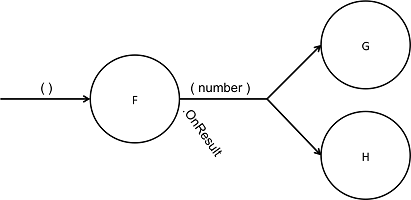
\includegraphics[width=.7\linewidth]{./img/diagramOut1to2.png}
	\caption{Ein Ausgang mehrere Empfänger}
\end{figure}


Falls ein Output an mehrere Empfänger weitergereicht werden soll, so gibt es
mehrere Möglichkeiten dies zu realisieren.
Die beste Möglichkeit ist, wenn die übergeordnete Integration den Rückgabewert
von F an die beiden nachfolgenden Funktionseinheiten einfach weiterreicht.
Eine weitere Möglichkeit wäre, wenn der Methode F ein Action mit übergeben wird,
und die übergeordnete Integration ruft G und H in einem Lambda auf.
Die dritte Möglichkeit besteht darin Events zu nutzen.
Leider bedarf es dann bei der Benutzung der API mehr Vorsicht, da man sich vorher auf ein Events registrieren muss, bevor man
die gewünschte Funktion aufrufen kann.

\begin{lstlisting}[caption= Mehrere Empfänger eines Outputs]
static void Main()
{ 
    var number = F();
    G(number);
    H(number);
}

static int F()
{
	return 42;
}

static void G(int number){}
static void H(int number){}
\end{lstlisting}




\subsubsection{Mehrere Output-Wege}

\begin{figure}[H]
	\centering
	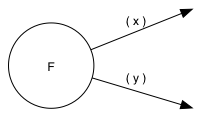
\includegraphics[width=.5\linewidth]{./img/diagramOut2.png}
	\caption{Eine Funktionseinheit mit mehreren Ausgängen}
\end{figure}



Wäre es für eine Operation erlaubt eine andere Funktionseinheit zu kennen, so
wäre es möglich die nachfolgenden Methoden per Namen innerhalb von \emph{F}
aufzurufen. Da aber Operationen entkoppelt von ihrer Umwelt sein sollen, geht das nicht.

Hat eine Funktionseinheit zwei Output-Wege, so gibt es zwei
Deutungsmöglichkeiten: Entweder kommen immer beide Daten x und y zurück oder
aber, es kann auch vorkommen, dass x und y nicht immer zurückgeben werden.
Im ersten Fall, wäre eine Umsetzung durch ein Tupel als Rückgabewert machbar.
Ist jedoch nicht gewährleistet, dass immer beide Werte zurückgeben werden, so
muss man in C\# die Outputwege als Actions über die Argumente der Methode
mitgeben. Somit werden die Verantwortlichkeiten bewahrt und die übergeordnete
Integration koordiniert weiter den Datenfluss. Die Operation selbst kennt nun keine
anderen Funktionseinheiten, sie weiß nur, dass sie zwei Ausgänge besitzt.

Ist diese Mehrdeutigkeit nicht erwünscht, so gibt es auch die Möglichkeit die den Kontrollfluss, auch in das Diagramm hier mit
dazu nehmen. Man kann in den Winkel der beiden Pfeile notieren, ob beide
Datenflüsse fließen, oder immer nur einer. 
Oft reicht es aber auch schon aus die Output-Wege zu benennen, damit ersichtlich
wird, ob es sich um ein \emph{and}, \emph{or} oder \emph{xor} handelt. Zum Beispiel würde ein \emph{onError}
und \emph{onSuccess} auf ein \emph{xor} hindeuten.

Alternativ könnte man auch hier Events nutzen, was aber durch das zusätzliche
Registrieren auf das Event nur in seltenen Fällen zu empfehlen ist.


Üblicherweise entstehen mehrere Output-Wege, sobald man eine
If-Else-Logik verwendet.

\pagebreak

Ein typischer Programmierstil in C\# veranschaulicht folgendes Beispiel:
\begin{lstlisting}[caption= {Typerischer Programmierstil, der nicht IOSP-konform ist}]
static void CheckAndSaveToFile(string inputstring)
{
   var filename = @"C:/test.txt";

   if(IsCorrectFormatted(inputstring))
      SaveStringToFile(inputstring, filename);
   else
      PrintError("Wrong Input Format");
}

static bool IsCorrectFormatted(string inputstring)
{
   bool isCorrectFormatted = false;

   // do string format checking here

   return isCorrectFormatted;
}
\end{lstlisting}

Eine komplizierte Bedingungsüberprüfung in eine separate Methode auszulagern
gilt als guter Programmierstil. Flow Design geht hier etwas weiter. Da es
untersagt ist, eine Kontrollstruktur und ein Methodenaufruf in einer
Methode zu kombinieren, besteht die Lösung darin, auch die If-Else-Anweisung in
die ausgelagerte Methode zu extrahieren und die zwei möglichen Ausgänge als Actions
in die Methode zu übergeben. Mithilfe der \enquote{Named Parameter} lässt sich die
Leserlichkeit weiter steigern (vor allem wenn es mehr als zwei Ausgänge
gibt, da man jedem Ausgang einen sinnvollen Namen geben kann).

\begin{lstlisting}[caption= {IOSP-konforme Variante}]
static void CheckAndSaveToFile(string inputstring)
{
   var filename = @"C:/test.txt";

   CheckIsCorrectFormat(inputstring, 
      onCorrect: () => SaveStringToFile(inputstring, filename);
      onError: () => PrintError("Wrong Input Format"));
}

static void CheckIsCorrectFormat(string inputstring, Action onCorrect, Action onError)
{
   bool isCorrectFormatted = false

   // do string format checking here

   if (isCorrectFormatted) 
      onCorrect();
   else
      onError();
}
\end{lstlisting}

Wie in diesem Beispiel zu erkennen ist, ist es möglich innerhalb eines
Lambdas auf lokale Variablen der übergeordneten Methode zuzugreifen. Dies
erlaubt es der Integration einer nachfolgenden Operation (hier \texttt{SaveStringToFile}) Parameter zu übergeben,
die die erste Operation (hier \texttt{CheckIsCorrectFormat}) selbst nicht kennt (hier
\texttt{filename} und auch \texttt{inputstring}). Die Operation ruft eine Action ohne
Parameter auf. Die Integration kann dadruch innerhalb des Lambda-Bodys frei
bestimmen, welche Methoden als nächstes aufgerufen werden.
Dadurch schränkt man die möglichen nachfolgenden Methodenaufrufe nicht durch
die Operation ein. In Sprachen die dieses Feature
nicht unterstützen, macht das die Umsetzung von Flow Design deutlich umständlicher.

\section{Auf Rückgabewert warten}

In C\# gibt es neben den \texttt{Actions} Methodenzeiger, die keine Rückgabewerte 
erlauben, auch Methodenzeiger, die einen Rückgabewert erlauben.
Diese werden mit\\\texttt{Func<Parameter,...,Rückgabewert>} deklariert.
Eine Methode die eine andere Methode über ein \texttt{Func} Methodenzeiger aufruft,
würde zwar das IOSP erfüllen - die Operation würde die andere Funktion nicht
kennen - jedoch würde trotzdem eine funktionale Abhängigkeit entstehen.
Aus diesem Grund ist das nachfolgende Beispiel nicht Flow Design konform.

\begin{lstlisting}[caption=Auf Rückgabewert warten]
static List<string> FormatStrings(List<string> lines , Func<string,string> formatFunc )
{
   List<string> result = new List<string>();
   foreach(line in lines)
   {
      string formattedstring = formatFunc(line);
      result.Add(formattedstring)
   }
   return result;
}
\end{lstlisting}


\section{Nutzen von IOSP}

Im diesem Abschnitt wird versucht zu erschließen was der Mehraufwand für die
Einhaltung des IOSP in der Praxis für einen Nutzen hat.
\subsubsection{Die Perlenkette}

Die Codebasis, die nach IOSP implementiert wurde, soll bildlich gesprochen einer
Perlenkette ähneln. Der Code besteht aus aneinandergereihte Funktionseinheiten,
die zusammen ein großes Ganzes bilden. Möchte man Änderungen an dem Programm
vornehmen, so brauch man nur an einer Stelle die Kette zu öffnen und etwas
hinzufügen oder entfernen. Danach schließt man die Kette wieder und das Programm
läuft wieder. Beim Einfügen oder Entfernen ist nur darauf zu achten, dass die
Eingänge und Ausgänge zueinander passen. Ist das nicht der Fall, so gibt es auch
die Möglichkeit eine s.g "Adapter"-Funktionseinheit zwischenzuschalten die die inkompatiblen
Ein- und Ausgänge zu korrigieren.Eine weitere Option wäre, die betroffenen
Funktionseinheiten und deren
ein- und ausgehenden Datentypen entsprechend abzuändern und die
Funktionseinheiten anzupassen.
Die erste Variante bringt möglicherweise einen Performanceverlust mit sich.
In vielen Stellen des Codes, ist dies jedoch meistens kein Problem.
Falls die Funktionseinheiten an anderer Stelle verwendet werden, oder sie zu
einer externen API gehören, ist möglicherweise eine Abänderung nicht
einfach umsetzbar. Dann bleibt nur die Option eine Adpater-Funktionseinheit zu verwenden.

\subsubsection{Funktionale Abhängigkeiten}

Funktionale Abhängigkeiten sind auch in anderen Gebieten außerhalb von der
Softwareentwicklung ein Problem. Dann wenn es darum geht produktive
Arbeitsabläufe zu gestalten.
Wenn jemand oder etwas seine Arbeit erst abschließen kann, wenn eine anderer
ihre Aufgabe erledigt hat, dann entsteht eine funktionale Abhängigkeit.
Solch eine Eigenschaft gilt es wenn möglich zu verhindern.
Besser ist es, wenn es Pool an Aufgaben gibt von dem sich jeder bedienen kann,
diese unabhängig von anderen Einheiten erledigen kann und dann das Ergebnis wieder
in ein Pool zurückgibt, von denen sich andere wiederum bedienen können.
Flow Design untersagt solche funktionale Abhängigkeiten in Operationen.
In der Praxis bewirkt das, dass die Operationen eine klare Aufgabe haben, welches
sie leichter zu testen macht.
Außerdem bleibt die Codebasis auch mit zunehmender Größe evolvierbar. Das
Zusammenspiel der Operationen bleibt leichter zu modifizieren, wodurch die
Codebasis an geänderte Anforderungen besser angepasst werden kann.

\section{Ausnahmen}

Generell gilt  wenn eine bewusste Entscheidung getroffen wird an einer Stelle gegen die IOSP
Regel zu verstoßen, ist das dann in Ordnung, solange sie gut überlegt ist und
die Auswirkungen in dem Fall keinen großen Einfluss haben.
Es gibt jedoch bereits einige Fälle, bei denen sich ein Aufheben der Regel als gut
herausgestellt hat.
\subsubsection{Rekursion}

Operationen ist es erlaubt sich selbst aufzurufen und wiederum auf das Ergebnis
zu warten. Besteht die Rekursion aus einer Kette an Operationen, so muss die letzte
Operation die erste Operation aufrufen und auf ihr Ergebnis warten dürfen.
\subsubsection{LINQ / Standard-Library Methoden}

Eine Koppelung an Methoden, die die Sprache selbst bereitstellt, hat keine
großen negativen Auswirkungen. Würde diese Ausnahme nicht gemacht werden, hätte
das zur Folge, dass unnötig viele Actions einer Methode mitgegeben werden
müssten. Beispiele von Methoden aus der Standardbibliothek von C\#:
\texttt{int.TryParse} , \texttt{List<>.Sort}, \texttt{Dictionary<>.Insert}, etc.

\subsubsection{UI-Logik}

Die UI-Logik ist von sich aus sehr state-behaftet und dadurch hat ein
konsequentes Einhalten des IOSP und Arbeiten mit Datenflüssen innerhalb des UI-Frameworks oft nur eine
Verkomplizierung des Codes zur Folge, ohne die Vorteile von IOSP wirklich zu
erhalten. Die Alternative besteht darin, die UI von der Businessdomäne/-logik zu
entkoppeln, sodass der Einfluss einer Nichteinhaltung keine Konsequenzen auf
die Businessdomäne hat.

Eine Herangehensweise besteht darin, die so genannte \emph{Interaktionen} des
UIs zu identifizieren. Diese Interaktionen bilden  die Schnittstelle
zwischen UI und Businessdomäne. Jede dieser Interaktionen stellt ein eigenes
Flow Design dar. Die Interaktionen und nachfolgende Methoden sind deshalb IOSP
konform. Das aktuelle Model des UIs wird einer Interaktion übergeben.
Dieses Model wird durch ein Flow Design modellierten Datenstrom modifiziert und am
Ende an die UI zurückgegeben. 
Die Aufgabe der UI-Logik besteht dann anschließend darin das Ergebnis der Modifikation des Models darzustellen.






\chapter{Die Entwurfsmethode}

Wie in der Einleitung dieser Arbeit bereits erwähnt, ist Flow Design nicht nur
ein Methodik um Datenflüsse auf dem Papier zu modellieren, sondern Flow Design
bietet neben dem Diagramm auch noch eine Entwurfsmethode um die Architektur einer Software
zu entwerfen.

\section{System-Umwelt-Diagramm}

Der erste Schritt beim Entwerfen einer Software nach Flow Design besteht
darin, die Grenzen des Systems kennenzulernen. Es soll herausgefunden
werden, welche Möglichkeiten es gibt, mit dem System zu interagieren und auf
welche Ressourcen das System zugreifen soll. Ziel soll sein, dass das System
so entworfen wird, dass die Businessdomäne entkoppelt bleibt von diesen
äußeren Faktoren.
Ein einfaches Schaubild soll einem helfen diese äußeren Faktoren zu
identifizieren: Ein Kreis wird in der Mitte eines Papiers gezeichnet, dieser
Kreis symbolisiert das System oder auch Domäne genannt.
Auf der linken Seite des Kreises werden die äußeren Systeme eingetragen, die
auf das System zugreifen und damit interagieren, diese Systeme oder
Techniken werden auch als Portale bezeichnet. Beispiele für Portale wären:
HTTP-Zugriff, Batch mode und GUIs.
Auf der anderen Seite des Kreises werden die externen Ressourcen eingetragen, auf die
das System Zugriff haben soll. Diese Ressourcen werden auch als Provider
bezeichnet. Ein Beispiel hierfür wären, ein Filesystem oder eine Datenbank.

Ralf Westphal bezeichnet diesen Kreis auch als Softwarezelle, was
verdeutlichen soll, dass das zu entwerfende System, sich wie eine Zelle in der
Natur verhalten soll. Eine Zelle weiß nicht viel über ihre Umwelt, sie befindet sich in
einer Nährstofflösung und verarbeitet die Stoffe, die durch ihre Membran in
ihr Inneres gelangen. Die Membran einer Softwarezelle trennt diese von
ihrer Umwelt (andere Systeme) und regelt den Austausch von Daten mit dem
Inneren des Systems. Ziel ist es später in der Implementierung darauf zu
achten, dass die "Schicht" oder "Membran", zwischen Domäne und Außenwelt möglichst
dünn bleibt.
Ist das System von der Umwelt entkoppelt lässt es sich besser testen und es
lassen sich leichter neue Portale und Provider an das System anhängen.

\section{Interfaceskizze ( im Falle einer GUI Anwendung )}

In Anlehnung an das User Experience Driven Development, soll schnell die
Features des Systems herausgefunden werden, die der Kunde wirklich
braucht. Es stellt sich heraus, das UML oder Use Cases für diese Aufgabe nur
bedingt hilfreich sind. Leichter für den Kunden zu verstehen ist eine
Interfaceskizze.
Diese soll gemeinsam mit der Kunden erarbeitet werden. Ein wichtiger Bestandteil
dieser Skizze besteht auch darin, die Interaktionen, die der
Nutzer mit dieser Oberfläche auslösen kann, zu identifizieren und zu benennen.

\section{Flow Design Entwurf}

Für jede der definierten Interaktionen aus der Interfaceskizze(n) wird ein Flow Design Flussdiagramm
erstellt.

Nachdem die Flow Design Diagramme erstellt wurden, muss überlegt werden, wie die
einzelnen Funktionseinheiten in Klassen, Dlls und Anwendungen zusammengefasst
und strukturiert werden sollen.
Dazu bietet sich an, einzelnen Funktionseinheiten zusätzlich mit dem Namen der
Klasse (gegebenenfalls auch DLLs und Anwendung) zu beschriften. Alternative ist es
auch üblich mehrere Funktionseinheiten mit einer gestrichelten Linien zu
umkreisen und auch mit unterschiedlichen Farben zu arbeiten, um die Gruppierungen und Zuordnungen zu verdeutlichen. 

Als letzter optionaler Schritt gilt es, Pfeile von solchen Datenströmen farblich hervorzuheben, die
parallel laufen können.

\section{Rekursive Eigenschaft}

Eine Softwarezelle hat die Eigenschaft, dass sie rekursive ist.
Das gesamte System lässt sich als eine große Softwarezelle betrachten, die wiederum
aus mehreren kleineren Softwarezellen bestehen können (Dlls und Anwendungen).
Diese Untersysteme sollen wieder wie das gesamte System möglichst entkoppelt
sein von den restlichen Untersystemen. Einer dieser Untersysteme muss sich dann
jedoch als integrierendes System verstehen, welches die anderen Untersysteme
kennt. Die Aufgabe dieses Untersystems besteht bestenfalls nur daraus, das
Zusammenspiel der Untersysteme zu koordinieren und keine komplexe Logik selbst zu implementieren.
Diese Untersysteme bestehen dann wieder aus Klassen und Methoden, die nach IOSP
implementiert sein sollen.
Somit könnte man selbst die Funktionseinheiten eines Flow Design
Flussdiagrammes als einzelne Softwarezellen betrachten.
Ralf Westphal behauptet, diese Architektur soll weniger starr und somit
universeller einsetzbar sein, als zum Beispiel das Schichtenmodell oder das Zwiebelschalenmodell.